%
% FH Technikum Wien
% !TEX encoding = UTF-8 Unicode
%
% Erstellung von Master- und Bachelorarbeiten an der FH Technikum Wien mit Hilfe von LaTeX und der Klasse TWBOOK
%
% Um ein eigenes Dokument zu erstellen, müssen Sie folgendes ergänzen:
% 1) Mit \documentclass[..] einstellen: Master- oder Bachelorarbeit, Studiengang und Sprache
% 2) Mit \newcommand{\FHTWCitationType}.. Zitierstandard festlegen (wird in der Regel vom Studiengang vorgegeben - bitte erfragen)
% 3) Deckblatt, Kurzfassung, etc. ausfüllen
% 4) und die Arbeit schreiben (die verwendeten Literaturquellen in Literatur.bib eintragen)
%
% Getestet mit TeXstudio mit Zeichenkodierung ISO-8859-1 (=ansinew/latin1) und MikTex unter Windows
% Zu beachten ist, dass die Kodierung der Datei mit der Kodierung des paketes inputenc zusammen passt!
% Die Kodierung der Datei twbook.cls MUSS ANSI betragen!
% Bei der Verwendung von UTF8 muss dnicht nur die Kodierung des Dokuments auf UTF8 gestellt sein, sondern auch die des BibTex-Files!
%
% Bugreports und Feedback bitte per E-Mail an latex@technikum-wien.at
%
% Versionen
% *) V0.7: 9.1.2015, RO: Modeline angepasst und verschoben
% *) V0.6: 10.10.2014, RO: Weitere Anpassung an die UK
% *) V0.5: 8.8.2014, WK: Literaturquellen überarbeitet und angepasst
% *) V0.4: 4.8.2014, WK: Initalversion in SVN eingespielt
%
\documentclass[Bachelor,BIF,english]{twbook}
\usepackage[utf8]{inputenc}
\usepackage[T1]{fontenc}

%
% Bitte in der folgenden Zeile den Zitierstandard festlegen
\newcommand{\FHTWCitationType}{IEEE} % IEEE oder HARVARD möglich - wenn Sie zwischen IEEE und HARVARD wechseln, bitte die temorären Dateien (aux, bbl, ...) löschen
%
\ifthenelse{\equal{\FHTWCitationType}{HARVARD}}{\usepackage{harvard}}{\usepackage{bibgerm}}

% Definition Code-Listings Formatierung:
\usepackage[final]{listings}
\lstset{captionpos=b, numberbychapter=false,caption=\lstname,frame=single, numbers=left, stepnumber=1, numbersep=2pt, xleftmargin=15pt, framexleftmargin=15pt, numberstyle=\tiny, tabsize=3, columns=fixed, basicstyle={\fontfamily{pcr}\selectfont\footnotesize}, keywordstyle=\bfseries, commentstyle={\color[gray]{0.33}\itshape}, stringstyle=\color[gray]{0.25}, breaklines, breakatwhitespace, breakautoindent}
\lstloadlanguages{[ANSI]C, C++, [gnu]make, gnuplot, Matlab}

%Formatieren des Quellcodeverzeichnisses
\makeatletter
% Setzen der Bezeichnungen für das Quellcodeverzeichnis/Abkürzungsverzeichnis in Abhängigkeit von der eingestellten Sprache
\providecommand\listacroname{}
\@ifclasswith{twbook}{english}
{%
    \renewcommand\lstlistingname{Code}
    \renewcommand\lstlistlistingname{List of Code}
    \renewcommand\listacroname{List of Abbreviations}
}{%
    \renewcommand\lstlistingname{Quellcode}
    \renewcommand\lstlistlistingname{Quellcodeverzeichnis}
    \renewcommand\listacroname{Abkürzungsverzeichnis}
}
% Wenn die Option listof=entryprefix gewählt wurde, Definition des Entyprefixes für das Quellcodeverzeichnis. Definition des Macros listoflolentryname analog zu listoflofentryname und listoflotentryname der KOMA-Klasse
\@ifclasswith{scrbook}{listof=entryprefix}
{%
    \newcommand\listoflolentryname\lstlistingname
}{%
}
\makeatother
\newcommand{\listofcode}{\phantomsection\lstlistoflistings}

% Die nachfolgenden Pakete stellen sonst nicht benötigte Features zur Verfügung
\usepackage{blindtext}
\usepackage{parskip}

%
% Einträge für Deckblatt, Kurzfassung, etc.
%
\title{Rebuilding a SharePoint 2013 Application with Angular 7 and Reactive Programming}
\author{Dominik Hack}
\studentnumber{1610257044}
\supervisor{DI Thomas Rongitsch}
\place{Vienna}
\kurzfassung{text}
\schlagworte{schlagwort1}
\outline{text}
\keywords{keyword1}

\begin{document}

%Festlegungen für den HARVARD-Zitierstandard
\ifthenelse{\equal{\FHTWCitationType}{HARVARD}}{
\bibliographystyle{Harvard_FHTW_MR}%Zitierstandard FH Technikum Wien, Studiengang Mechatronik/Robotik, Version 1.2e
\citationstyle{dcu}%Correct citation-style (Harvardand, ";" between citations, "," between author and year)
\citationmode{abbr}%use "et al." with first citation
\iflanguage{ngerman}{
    %Deutsch Neue Rechtschreibung
    \newcommand{\citepic}[1]{(Quelle: \protect\cite{#1})}%Zitat: Bild
    \newcommand{\citefig}[2]{(Quelle: \protect\cite{#1}, S. #2)}%Zitat: Bild aus Dokument
    \newcommand{\citefigm}[2]{(Quelle: modifiziert "ubernommen aus \protect\cite{#1}, S. #2)}%Zitat: modifiziertes Bild aus Dokument
    \newcommand{\citep}{\citeasnoun}%In-Line Zitiat entweder mit \citep{} oder \citeasnoun{}
    \newcommand{\acessedthrough}{Verf{\"u}gbar unter:}%Für URL-Angabe
    \newcommand{\acessedthroughp}{Verf{\"u}gbar bei:}%Für URL-Angabe (Geschützte Datenbank, Zugriff durch FH)
    \newcommand{\acessedat}{Zugang am}%Für URL-Datum-Angabe
    \newcommand{\singlepage}{S.}%Für Seitenangabe (einzelne Seite)
    \newcommand{\multiplepages}{S.}%Für Seitenangabe (mehrere Seiten)
    \newcommand{\chapternr}{K.}%Für Kapitelangabe
    \renewcommand{\harvardand}{\&}%Harvardand in Zitaten
    \newcommand{\abstractonly}{ausschließlich Abstract}
    \newcommand{\edition}{. Auflage}%Angabe der Auflage
}{
\iflanguage{german}{
    %Deutsch
    \newcommand{\citepic}[1]{(Quelle: \protect\cite{#1})}%Zitat: Bild
    \newcommand{\citefig}[2]{(Quelle: \protect\cite{#1}, S. #2)}%Zitat: Bild aus Dokument
    \newcommand{\citefigm}[2]{(Quelle: modifiziert "ubernommen aus \protect\cite{#1}, S. #2)}%Zitat: modifiziertes Bild aus Dokument
    \newcommand{\citep}{\citeasnoun}%In-Line Zitiat entweder mit \citep{} oder \citeasnoun{}
    \newcommand{\acessedthrough}{Verf{\"u}gbar unter:}%Für URL-Angabe
    \newcommand{\acessedthroughp}{Verf{\"u}gbar bei:}%Für URL-Angabe (Geschützte Datenbank, Zugriff durch FH)
    \newcommand{\acessedat}{Zugang am}%Für URL-Datum-Angabe
    \newcommand{\singlepage}{S.}%Für Seitenangabe (einzelne Seite)
    \newcommand{\multiplepages}{S.}%Für Seitenangabe (mehrere Seiten)
    \newcommand{\chapternr}{K.}%Für Kapitelangabe
    \renewcommand{\harvardand}{\&}%Harvardand in Zitaten
    \newcommand{\abstractonly}{ausschließlich Abstract}
    \newcommand{\edition}{. Auflage}%Angabe der Auflage
}{
    %Englisch
    \newcommand{\citepic}[1]{(Source: \protect\cite{#1})}%Zitat: Bild
    \newcommand{\citefig}[2]{(Source: \protect\cite{#1}, p. #2)}%Zitat: Bild aus Dokument
    \newcommand{\citefigm}[2]{(Source: taken with modification from \protect\cite{#1}, p. #2)}%Zitat: modifiziertes Bild aus Dokument
    \newcommand{\citep}{\citeasnoun}%In-Line Zitiat entweder mit \citep{} oder \citeasnoun{}
    \newcommand{\acessedthrough}{Available at:}%Für URL-Angabe
    \newcommand{\acessedthroughp}{Available through:}%Für URL-Angabe (Geschützte Datenbank, Zugriff durch FH)
    \newcommand{\acessedat}{Accessed}%Für URL-Datum-Angabe
    \newcommand{\singlepage}{p.}%Für Seitenangabe (einzelne Seite)
    \newcommand{\multiplepages}{pp.}%Für Seitenangabe (mehrere Seiten)
    \newcommand{\chapternr}{Ch.}%Für Kapitelangabe
    \renewcommand{\harvardand}{\&}%Harvardand in Zitaten
    \newcommand{\abstractonly}{Abstract only}
    \newcommand{\edition}{~edition}%Edition -> note, that you have to write "edition = {2nd},"!
}}}

\maketitle
\chapter{Introduction}
describe starting point, why will this project be realised, what should be achieved?, motivation, SharePoint \cite{SharePoint}, SharePoint Requirements (IE), Project Requirements (features), old solution, rebuilding with angular because of new features and same cost of developing a new application and not building on sharepoint feature (also extensibility, maintenance and encapsulation), better for company to have knowledge in Angular than in Sharepoint 2013 (because more projects also use angular), possible research questions: extensibility (1 of 4 team members have experience in developing sharepoint apps, 3 of 4 team members have experience in developing angular apps), maintenance?, observer patter in reactive programming?, overhead of redux?, war angular wirklich schneller zu entwickeln als sharepoint? (Vorteile: Angular wird häufig auch bei anderen Projekten verwendet, no publishing of whole sharepoint project through hosting angular app locally which saves time also angular supports hot reloading)
\clearpage


\chapter{Tools \& Frameworks} 
what will be presented in this chapter (reactive programming; tools to use this paradigm with: ReactiveX, Redux and NgRx; Angular; why typescript; what components are; introduction of important tools used by angular: npm, webpack and babel),
For the implementation of this project a technology had to be decided on that meets the requirements of being integrated into and communicate with SharePoint 2013.

\section{Reactive Programming}
If an interaction with a reactive application takes place, a event occurs which the software will respond on by reacting on it in a certain way. Therefore a reactive software system could be any application with a graphical user interface (GUI) reacting on user input, a network monitoring service reacting on certain changes of the network or even a simple calculator reacting on button presses. reactive applications can become complex because of a mixed combination of data and control flow \cite[p.~1]{PositivEffectOfRP}, 
two main approaches to implement a reactive application (also explain figure):
\begin{figure}[!htbp]
\centering
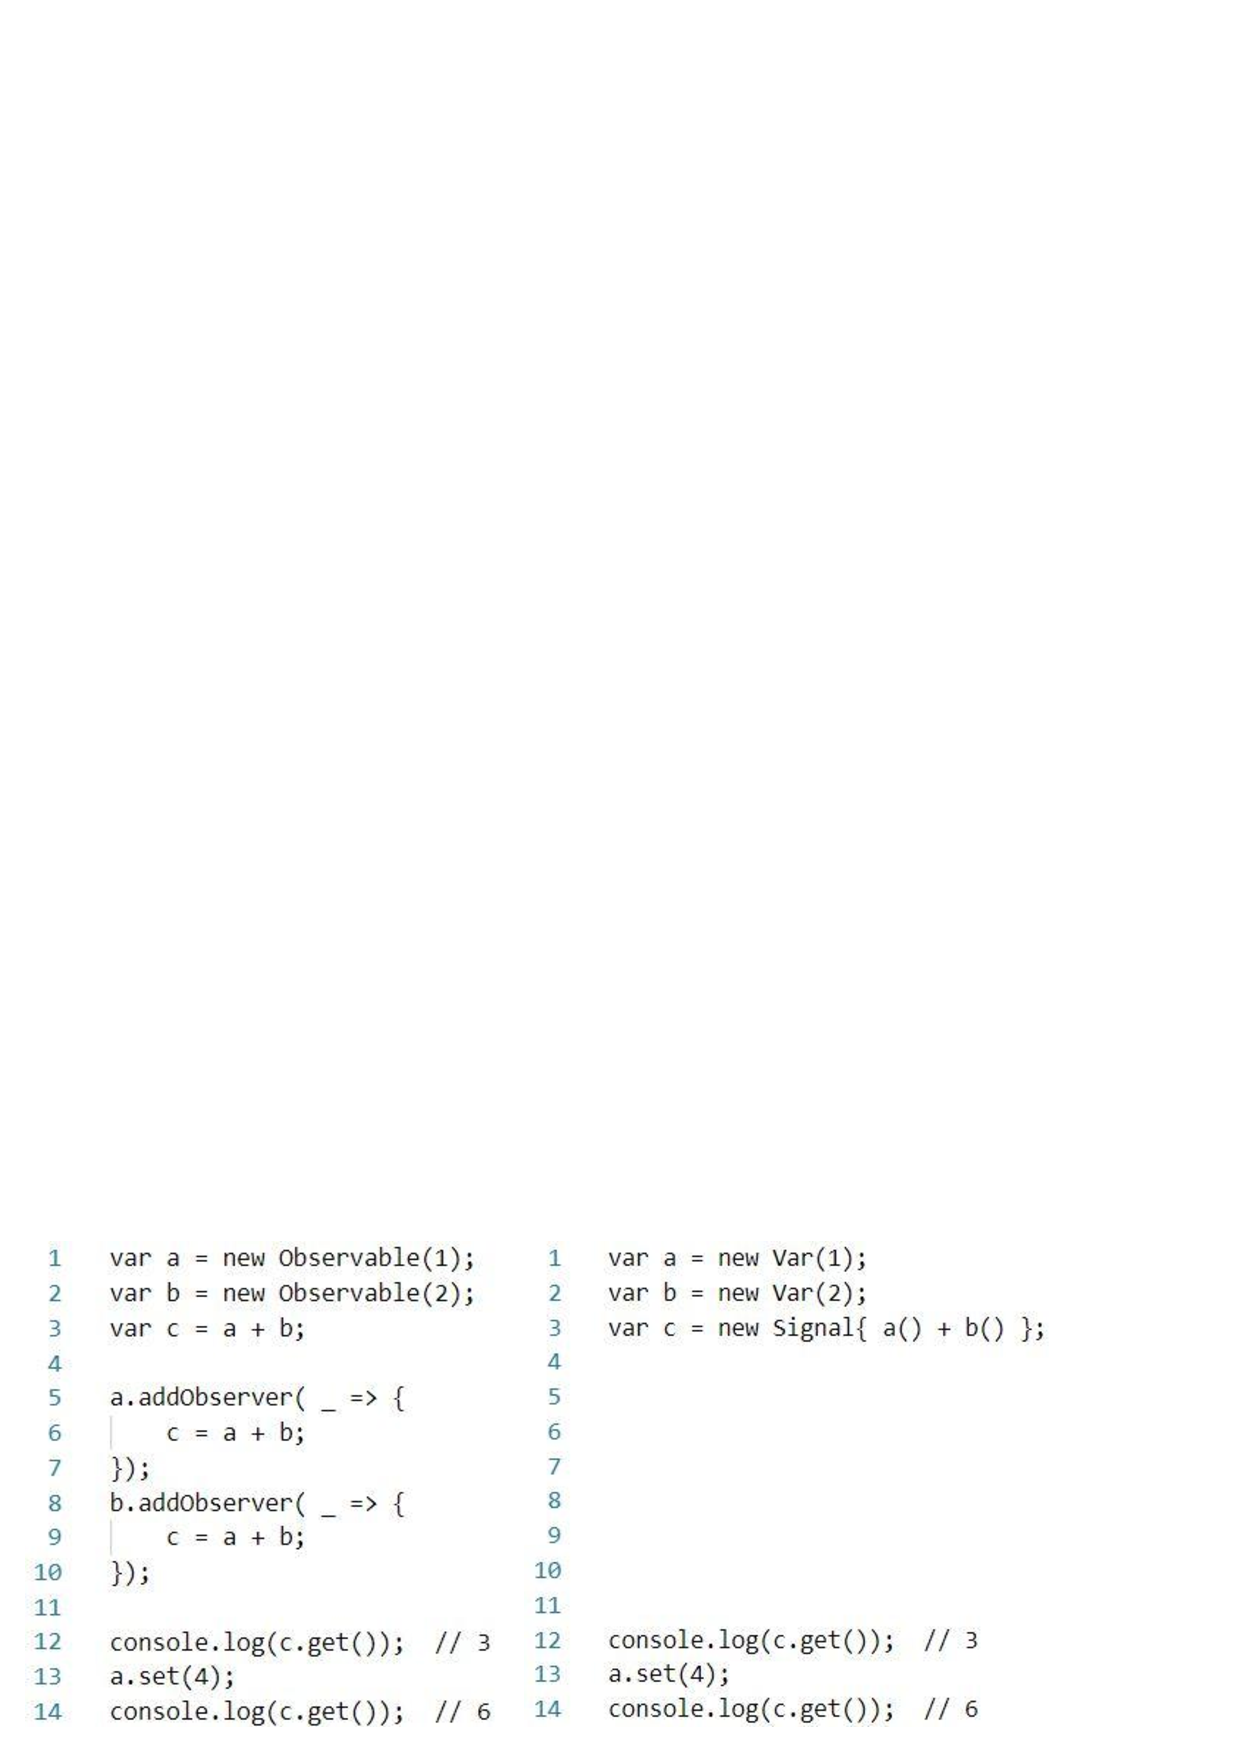
\includegraphics[width=0.75\linewidth]{PICs/pseudo_Code_reactive_2_ways.png}
\caption{JavaScript-like pseudo code of the observer pattern approach (left) and the signals and vars approach (right) \cite[p.~797]{DebuggingRP} \cite[p.~3]{PositivEffectOfRP}}\label{Fig1}
\end{figure}
traditional approach observer pattern \cite[p.~360-372]{ObserverDP}, decouples event consumers from event producers \cite[p.~953]{RPWalkthrough}, (in object oriented programming using observer pattern, decouples observers or subscribers from observables or subjects, observers subscribe to observables, observables do not know their subscribers, when observables change their state they notify their observers depending on the implementation this can be done through emitting events. When a subscriber learns of a change in the state of the subject, he adjusts his state to that of the subject. \cite[p.~363]{ObserverDP}),
vs the other way, what is reactive programming: programming paradigm supporting language-level abstractions \cite[p.~953]{RPWalkthrough}, The four principles all implementations of reactive programming pursue are:
\begin{itemize}
\item Declarativeness: declaring how the states of the components depend on each other, not how to retrieve the state when changes occur \cite[p.~2]{PositivEffectOfRP}.
\item Abstraction over change propagation: No need to manually update dependencies, propagation of change is handled by language runtime \cite[p.~2]{PositivEffectOfRP}.
\item Composability: Composing reactive computations through abstractions \cite[p.~2]{PositivEffectOfRP}.
\item Favoring data flow over control flow: Calculations of the software system are triggered by new data or events and are not depending on the execution of the control flow \cite[p.~2]{PositivEffectOfRP}.
\end{itemize}
einiges an Forschung wurde schon betrieben und nach der Einführung von funcitonal reactive programming in Haskell wurde dieses konzept auch in Scheme (FrTime \cite{FrTime}), Scala (Scala.react \cite{DeprecatingOP}) und JavaScript (Flapjax \cite{Flapjax}) implementiert, sogar wurde in Microsofts Reactive Extensions (RX or ReactiveX) konzepte von reactive programming implementiert \cite[p.~954]{RPWalkthrough} \cite[p.~796]{DebuggingRP} \cite[p.~2]{PositivEffectOfRP}
(signals or behaviours: time changing values, treated as constraints of the language runtime, when an inconcistency of a signal or behaviour is detected a recalculation is triggered \cite[p.~797]{DebuggingRP} \cite[p.~3]{PositivEffectOfRP}, can either depend on other signals or vars, vars are reactive values like signals but without dependencies \cite[p.~2]{PositivEffectOfRP}), less error prone, easier to understand, still immature field -> lack of developer tools like debuggers \cite[p.~796]{DebuggingRP} 
\subsection{ReactiveX}
general introduction (what is it \cite{ReactiveExtensions} (von Microsoft aber open source), why should it be used), \cite{ReactiveX}, bringing functional-reactive-programming-like reactivity 
observables, observables background with reactor pattern \cite{RxObservables}
\subsection{Redux}
general introduction (what is it, why should it be used), \cite{Redux}, motivation why redux \cite{ReduxIntroMoti}, core concept \cite{ReduxIntroCC}, three principles \cite{ReduxIntro3P}, figure for explanation
\subsection{NgRx}
general introduction (what is it, why should it be used), \cite{Ngrx}, ng/store, effects

\section{Angular}
what is angular?, what is it for?, dependency injection, data binding, \cite[p.~]{YakovFainAngular}
\subsection{TypeScript}
general introduction (what is it, why should it be used), 
\subsection{Components}
general introduction (what is it, why should it be used), 
\subsection{npm}
general introduction (what is it, why should it be used), 
tool to install everything js based
\subsection{Webpack}
general introduction (what is it, why should it be used), 
bundling assets (vendor, main, styles, etc.)
\subsection{Babel}
general introduction (what is it, why should it be used), 
polyfills
\clearpage 

\chapter{Implementation}
The following sections deal with describing the processes utilized to ensure the quality of the final product both during the development phase and after completion. First, the general procedures related to project management and continuous integration are illustrated. Subsequently, the software architecture including the project structure, the interfaces and additionally added technologies as well as methodologies will be presented. Finally, the development with reactive programming is discussed.

\section{Project Management}
To successfully complete this project with as few errors as possible and to develop a product that adds business value to the customer and satisfies the customers' needs, the agile project management framework "Scrum" \cite{Scrum} was employed. The scrum team consisted of 3 developers, one of whom was one half of his time involved in scrum master activities, and one product owner. The product owner took care of analyzing the current problems together with the customer in order to develop a possible solution. Based on these requirements, a first version of the backlog was created to give the development team an overview of the product to be developed. Subsequently, the developer team estimated the story points of each user story using planning poker. With this information the product owner calculated the offer for the customer. After the contract was signed scrum team met for a project kick-off meeting to discuss the highest priority user stories.
\\[\baselineskip]
The length of a sprint for this project was one week, since at first the user stories were small enough so that the commitment to the sprint goal could be kept. Later, the length of a sprint was increased to two weeks, because on the one hand some user stories were too large to finish in a week and on the other hand a developer had to be assigned to other projects for some time. Sprints were planned using the user-story or task-board tools provided by the company's TFS (Team Foundation Server) \cite{TFS}.
Every day a daily stand-up was held where each developer announced the current status of their user stories. If there was any difficulty implementing a user story, after the meeting, the task in question was discussed with at least one other developer. If no solution was found, the product owner was contacted to discuss the problem.
what happens when a user story is finished, explain technical details below everything else in here (pull request, code review, resolving user story with product owner), reviewing why a commitment could not be kept 

\section{Continuous Integration}
CI Process (figure of pipeline, start via pushing the changes to the git \cite{Git} repository, pull request with code review one other developer has to approve, restore, building of pushed branch through separate build servers, executing all unit tests if failure pull request will be rejected till next push), TFS (with repository, ui for ci pipeline), user acceptance test server for customer to test application before deployment to production occurs, dev server for developer to test released application, continous deployment not possible because of sharepoint (flo bzw. tobi fragen)

\section{Integrating Angular in SharePoint 2013}
Microsoft Docs about the script editor webpart for the development process, real integration in sharepoint through a sharepoint feature,

\section{Software Architecture}

\subsection{Software Components}
alert, blog, core, entities, services, service entities, shared, containers, components, routing (router, guard); figure of project structure;

\subsection{Interfaces}
pnpjs, "REST" API, JSOM, CSOM, own backend in sharepoint, figure about how the communication between angular and sharepoint looks like

\subsection{Styles}
SASS, BEM

\section{Reactive Programming}

\subsection{Libraries \& Development Tools}
rxjs, easier use of the redux pattern, more features for reactive programming, chrome extension

\subsection{Adding a new Feature}
explain implementation in form of an example like "showing blog entry", Store, Actions, State, Reducer, Selector, Effect, etc., 

\subsection{Unit Testing}
testing with reactive programming; karma;

\clearpage


\chapter{Discussion}

\section{Development}
Difficulties, possible overhead of Redux huge advantages at a cost (also extensions for chrome which makes debugging less painful)

\section{Results}
presenting finished solution
\clearpage


\chapter{Conclusion \& Future Work}




% Hier beginnen die Verzeichnisse.
\clearpage
\ifthenelse{\equal{\FHTWCitationType}{HARVARD}}{}{\bibliographystyle{gerabbrv}}
\bibliography{Literatur}
\clearpage

% Das Abbildungsverzeichnis
\listoffigures
\clearpage

\listofcode
\clearpage

\phantomsection
\addcontentsline{toc}{chapter}{\listacroname}
\chapter*{\listacroname}
\begin{acronym}[XXXXX]
    \acro{CLI}[CLI]{Command-Line Interface}
    \acro{TFS}[TFS]{Team Foundation Server}
    \acro{API}[API]{Application Programming Interface}
    \acro{ECMA}[ECMA]{European Computer Manufacturers Association}
    \acro{W3C}[W3C]{World Wide Web Consortium}
    \acro{HTML}[HTML]{Hypertext Markup Language}
    \acro{CSS}[CSS]{Cascading Style Sheets}
    \acro{DOM}[DOM]{Document Object Model}
    \acro{UI}[UI]{User Interface}
\end{acronym}

\end{document}}